\documentclass[11pt, oneside]{article}   	% use "amsart" instead of "article" for AMSLaTeX format
\usepackage{geometry}                		% See geometry.pdf to learn the layout options. There are lots.
\usepackage{amsmath}

\geometry{letterpaper}                   		% ... or a4paper or a5paper or ... 
%\geometry{landscape}                		% Activate for for rotated page geometry
%\usepackage[parfill]{parskip}    		% Activate to begin paragraphs with an empty line rather than an indent
\usepackage{graphicx}				% Use pdf, png, jpg, or eps with pdflatex; use eps in DVI mode
								% TeX will automatically convert eps --> pdf in pdflatex		
\usepackage{amssymb}
\usepackage{amsmath}
\usepackage{parskip}

\graphicspath{{/Users/telliott_admin/Dropbox/Tex/png/}}

\title{Rotation matrix simplified}
%\author{The Author}
\date{}							% Activate to display a given date or no date

\begin{document}
\maketitle
%\subsection{}
\Large
\noindent
Our goal here is to find the equations for rotation of coordinates.  We want to be as simple as we can, so that we can remember how the derivation works.  We will need a couple of preliminary facts, however.

\begin{itemize}
\item a procedure to compute the dot product of two vectors
\item when vectors are perpendicular (orthogonal) $\iff$ the dot product is zero
\item the projection of a vector onto any other vector is just the dot product, with the second vector re-scaled (normalized) to have unit length
\item a rotated set of coordinates is a set of orthogonal unit vectors (in whatever direction we choose)
\end{itemize}

I have written extensively about the dot product elsewhere.  It is a number computed from the components of any two vectors $\mathbf{a}$ and $\mathbf{b}$ by the following procedure:
\[ \mathbf{a} \cdot \mathbf{b} = a_1 b_1 + a_2 b_2 + \dots + a_n b_n \]

For example
\[ \langle 3, 2 \rangle \cdot  \langle 2, 5 \rangle = 3 \times 2 + 2 \times 5 = 16 \]
\[ \langle 1, 0 \rangle \cdot  \langle 0, 1 \rangle = 0 \]
\[ \langle \cos \theta, \sin \theta \rangle \cdot  \langle -\sin \theta, \cos \theta \rangle = 0 \]

As we might expect, the unit vector along the $x$-axis, usually called $\hat{\mathbf{i}}$, and the unit vector along the $y$-axis, $\hat{\mathbf{j}}$, are perpendicular to each other.  Similarly, for any angle $\theta$, the given vectors $\langle \cos \theta, \sin \theta \rangle$ and $\langle -\sin \theta, \cos \theta \rangle$ are perpendicular.

Furthermore, the length of a vector $\mathbf{a}$ is represented as $|\mathbf{a}|$, or even just $a$, and the length squared is

\[ a^2 = \mathbf{a} \cdot \mathbf{a} \]

With respect to the projection, an example should also make that clearer.  Suppose we are working with two-dimensional vectors and we decide that our new $x$-axis should be in the direction of the vector $3,4$.  The first thing to do is to re-scale this to be a unit vector.  The length squared is
\[ \langle 3, 4 \rangle \cdot  \langle 3, 4 \rangle = 9 + 16 = 25 \]

Hence the length is $5$ and our new unit vector $\mathbf{u}$ is 
\[ \mathbf{u} = \langle 3/5, 4/5 \rangle \]

We also need a unit vector $\mathbf{v}$ such that $\mathbf{u} \cdot \mathbf{v} = 0$.  Hence
\[ \mathbf{v} = \langle -4/5, 3/5 \rangle \]
or 
\[ \mathbf{v} = \langle 4/5, -3/5 \rangle \]
These two vectors are the same vector, just pointing in opposite directions (which is in the same direction, for the purpose of vectors).

Then for \emph{any} vector $\mathbf{a}$, we can compute the same vector in a set of rotated coordinates based on $\mathbf{u}$ and $\mathbf{v}$ as
\[ a_u = \mathbf{a} \cdot \mathbf{u} \]
\[ a_v = \mathbf{a} \cdot \mathbf{v} \]

\subsection*{derivation}

All we have to do is to think about rotation of the unit vectors $\hat{\mathbf{i}}$ and $\hat{\mathbf{j}}$ through an angle $\theta$ counter-clockwise.  

Start with $\hat{\mathbf{i}}$.  The new vector we seek is still a unit vector, but rotated so that it forms an angle $\theta$ with the positive $x$-axis.

The new vector has both $\hat{\mathbf{i}}$ and $\hat{\mathbf{j}}$ components. Projection onto $\hat{\mathbf{i}}$ gives a vector with unit length times $\cos \theta$ or just $\cos \theta$, and similarly, the projection onto $\hat{\mathbf{j}}$ gives a length $\sin \theta$.  Clearly the squared length is $\cos^2 \theta + \sin^2 \theta$, so this is a unit vector.

In vector notation we would say that
\[ \langle 1,0 \rangle \ \Rightarrow \ \langle \cos \theta, \sin \theta \rangle \]
In matrix language the two vectors are related in this way:
\[
\begin{bmatrix}  
1  \\  
0  
\end{bmatrix}
\Rightarrow
\begin{bmatrix}  
\cos\  \theta  \\  
\sin\  \theta  
\end{bmatrix}
\]
So the question is, what matrix will multiply $\hat{\mathbf{i}}$ to give this result?
\[
\begin{bmatrix}  
a & b  \\  
c & d  
\end{bmatrix}
\begin{bmatrix}  
1  \\  
0  
\end{bmatrix}
=
\begin{bmatrix}  
\cos\  \theta  \\  
\sin\  \theta  
\end{bmatrix}
\]
Recall that matrix multiplication works like this
\begin{center} 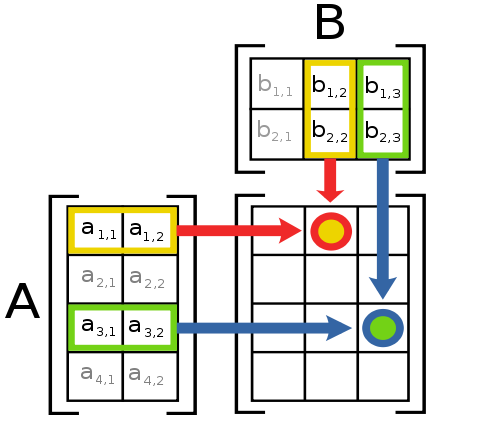
\includegraphics [scale=0.35] {mm1.png} \end{center}

For a matrix times a vector, $B$ would have only a single column.

So going back to this:

\[
\begin{bmatrix}  
a & b  \\  
c & d  
\end{bmatrix}
\begin{bmatrix}  
1  \\  
0  
\end{bmatrix}
=
\begin{bmatrix}  
\cos\  \theta  \\  
\sin\  \theta  
\end{bmatrix}
\]


I hope it's pretty clear that $a = \cos \theta$ and $c = \sin \theta$:
\[
\begin{bmatrix}  
\cos \theta & b  \\  
\sin \theta & d  
\end{bmatrix}
\begin{bmatrix}  
1  \\  
0  
\end{bmatrix}
=
\begin{bmatrix}  
\cos\  \theta  \\  
\sin\  \theta  
\end{bmatrix}
\]
Can you see why this is true?

On the other hand, rotation of the unit $\hat{\mathbf{j}}$ vector by $\theta$ should give
\[
\begin{bmatrix}  
a & b  \\  
c & d  
\end{bmatrix}
\begin{bmatrix}  
0  \\  
1  
\end{bmatrix}
=
\begin{bmatrix}  
-\sin \  \theta  \\  
\ \ \cos \  \theta  
\end{bmatrix}
\]
The minus sign comes because the new vector is now sticking out into the second quadrant.

Again, it should be clear that 
\[
\begin{bmatrix}  
a & -\sin \  \theta  \\  
c & \ \ \cos \  \theta  
\end{bmatrix}
\begin{bmatrix}  
0  \\  
1  
\end{bmatrix}
=
\begin{bmatrix}  
-\sin \  \theta  \\  
\ \ \cos \  \theta  
\end{bmatrix}
\]

Now, just put them together:
\[
R_{ccw} = 
\begin{bmatrix}   \ \cos \theta & -\sin \theta  \\  \ \sin \theta & \ \ \cos \theta  \end{bmatrix}
\]
\[
\begin{bmatrix}   \ \cos \theta & -\sin \theta  \\  \ \sin \theta & \ \ \cos \theta  \end{bmatrix}
\begin{bmatrix}   x   \\  y  \end{bmatrix} = \begin{bmatrix}   u   \\  v  \end{bmatrix}
\]
In particular, a rotation of $90^{\circ}$ ccw goes like this
\[
\begin{bmatrix}   0 & -1  \\  1 & \ \ 0  \end{bmatrix}
\begin{bmatrix}   1   \\  0  \end{bmatrix} = \begin{bmatrix}   0   \\  1  \end{bmatrix}
\]
$\hat{\mathbf{i}}$ is rotated to become $\hat{\mathbf{j}}$.

I claim that since the matrix we found works for both of the unit vectors it will work for any vector, since any vector can be written as a linear combination of the unit vectors
\[ \mathbf{a} = a_1 \ \hat{\mathbf{i}} + a_2 \ \hat{\mathbf{j}} \]

The inverse of the matrix we derived would be used for clockwise rotation and it is just
\[
R_{cw} =
\begin{bmatrix}   \ \ \ \cos \theta & \ \sin \theta  \\  -\sin \theta & \ \ \cos \theta  \end{bmatrix}
\]
You can verify this by remembering the rule for $2 \times 2$ or by multiplication
\[
R_{cw} \  R_{ccw} =
\begin{bmatrix}   \ \ \ \cos \theta & \ \sin \theta  \\  -\sin \theta & \ \ \cos \theta  \end{bmatrix}
\begin{bmatrix}   \ \cos \theta & -\sin \theta  \\  \ \sin \theta & \ \ \cos \theta  \end{bmatrix}
= 
\begin{bmatrix}   1 & 0  \\  0 & 1 \end{bmatrix}
= I
\]
Don't be confused when someone talks about rotation of the coordinate system.  Here, the coordinate system stayed fixed but we rotated the vector counter-clockwise.  We achieve the same thing (and use the same equation) for a \emph{clockwise} rotation of the coordinate system through an angle $\theta$.

If you really want to rotate the coordinate system counter-clockwise, rotate the vector clockwise.

\subsection*{consequence}

One other neat thing comes out of this when we ask about rotation by an angle $s + t$.  We can write two equivalent expressions, one by substituting $\theta=s+t$, and the other by doing two sequential applications of the matrix.  That is:
\[
\begin{bmatrix}   \ \cos (s+t) & -\sin (s+t)  \\  \ \sin (s+t) & \ \ \cos (s+t)  \end{bmatrix} =
\begin{bmatrix}   \ \cos s & -\sin s  \\  \ \sin s & \ \ \cos s  \end{bmatrix}
\begin{bmatrix}   \ \cos t & -\sin t  \\  \ \sin t & \ \ \cos t  \end{bmatrix}
\]
Look at the term on the upper-left, $\cos(s+t)$.  Sound familiar?  Carry out the matrix multiplication on the right for that element
\[ \cos(s+t) = \cos s \cos t - \sin s \sin t \]
We have derived the cosine addition formula.  Similarly, the bottom-left term is for the sine
\[ \sin(s+t) = \sin s \cos t + \cos s \sin t \]

\subsection*{standard derivation}
Here is a sort of minimalist diagram of rotation
\begin{center} 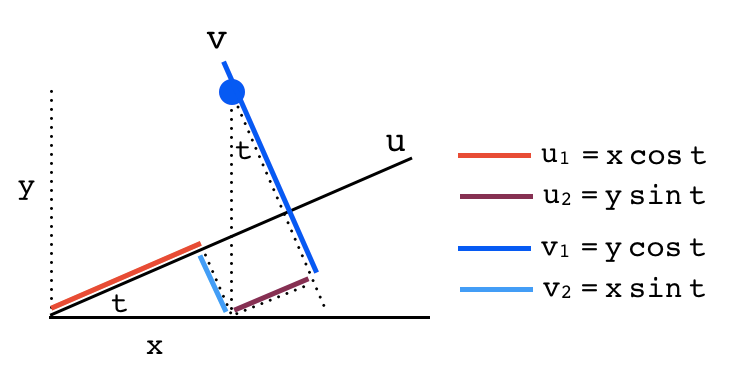
\includegraphics [scale=0.5] {min_rotation.png} \end{center}

We draw the horizontal $x$-axis and the rotated $u$-axis.  The angle between them is $t$.  We plot our point and then draw perpendiculars to both axes.  To finish the set-up, we draw perpendiculars from the point $(x,0)$ as shown.

Once the drawing is rendered, we are almost done.  You will know that you've done it right if you have both $x$ and $y$ as the \emph{hypotenuse of a right triangle}.  Now we just work our way through

\[ u_1 = x \cos t \]
\[ u_2 = y \sin t \]

(Any small angle in the diagram is $t$.  Can you prove it?)

So 
\[ u = x \cos t + y \sin t \]
\[ v_1 = y \cos t \]
Finally, 
\[ v_2 = x \sin t \]
\[ v = -  x \sin t + y \cos t \]
Rewriting this result using vector notation with the traditional angle symbol $\theta$
\[
\begin{bmatrix}   \ \ \ \ \cos \theta & \sin \theta  \\  \ -\sin \theta & \ \cos \theta  \end{bmatrix}
\begin{bmatrix}   x   \\  y  \end{bmatrix} = \begin{bmatrix}   u   \\  v  \end{bmatrix}
\]
As mentioned above, a point of confusion that often arises with these formulas is the distinction between rotating a vector and rotating the axes or coordinate system..  The derivation above is for a rotation of the axes counter-clockwise.  This is equivalent to rotating the point clockwise.  If, instead we were to rotate the point counter-clockwise, the rotation matrix $R_{ccw}$ would be
\[
\begin{bmatrix}   \ \ \cos \theta & -\sin \theta  \\  \ \sin \theta & \ \ \cos \theta  \end{bmatrix}
\begin{bmatrix}   x   \\  y  \end{bmatrix} = \begin{bmatrix}   u   \\  v  \end{bmatrix}
\]
\subsection*{yet another way}
We can look at this in still a different way.  Write
\[
\begin{bmatrix}  x \\ y \end{bmatrix}
=
x
\begin{bmatrix}  1 \\ 0 \end{bmatrix}
+
y
\begin{bmatrix}  0 \\ 1 \end{bmatrix}
\]
In this representation, the vector $<x,y>$ is a linear combination of the unit vectors $\hat{i}=\ <1,0>$ and $\hat{j}=\ <0,1>$.

To rotate the point, we just want to use a different set of unit vectors.  The new unit vectors (for the rotated axes) are $<\cos \theta,\sin \theta>$ and $<-\sin \theta,\cos \theta>$.  

If you compute their lengths, it is clear that they are, in fact, unit vectors.
\[
\begin{bmatrix}  x' \\ y' \end{bmatrix}
=
x
\begin{bmatrix}  \cos \theta \\ \sin \theta \end{bmatrix}
+
y
\begin{bmatrix}  -\sin \theta \\ \ \ \cos \theta \end{bmatrix}
\]
Written as a matrix multiplication, this is
\[
\begin{bmatrix}  x' \\ y' \end{bmatrix}
=
\begin{bmatrix}  
\cos \theta & -\sin \theta \\
\sin \theta & \ \  \cos \theta 
\end{bmatrix}
\begin{bmatrix}  x \\ y \end{bmatrix}
\]
\end{document}  